We will now examine the details of monoclonal antibody production.
It is done in multiple steps, as summarized on figure \ref{fig:Monoclonal_Antibody_Production}.

\begin{figure}[H]
    \begin{center}
        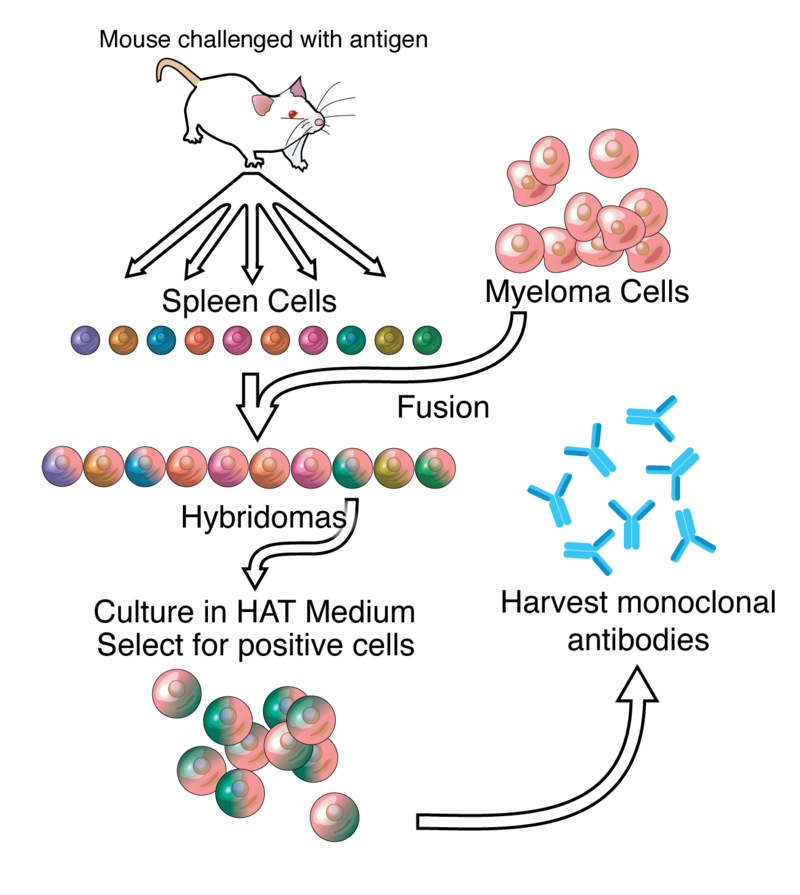
\includegraphics[width=0.4\textwidth]{../Images/mab_hybridomas.png}
        \caption{Monoclonal antibody production}
        \label{fig:Monoclonal_Antibody_Production}
    \end{center}
\end{figure}


\subsubsection{Step 1 : Immunization}

In order to begin the production of monoclonal antibodies, it is first
needed to immunize an animal with the antigen of interest. Typically, 
mice are used for this process \cite{leenaars_critical_2005}. 
An \emph{immunogen}, \textit{i.e} an antigen due to induce an immune response
in the animal, is then injected into the animal, along with an adjuvant
aiming at enhancing the immune response.


\subsubsection{Step 2 : Fusion and selection}

Once the animal has had sufficient time to develop a good immune
response to the antigen it was injected with, its splenic B-cells
that produce antibodies specific to the antigen are collected.

On their own, these B-cells coming from the animal's spleen produce
monoclonal antibodies ; however, we cannot stop the process there
as these cells have a limited life expectancy and thus cannot be
use in an industrial process without having to restart the immunization
stage frequently with new animals.

Thus, a technique called \emph{fusion}, invented by G. Köhler and
C. Milstein in 1975 \cite{kohler_continuous_1975} is used to immortalize
the B-cells of interest. In order to do so, these cells are fused with
compatible myeloma cells, which are cancerous cells -- and thus immortal.

It should be noted that as cells have two ways of producing naturally
nucleotides : by the \emph{de novo} pathway, and by a salvage way using the enzyme
hypoxanthine guanine phosphoribosyl transferase (HGPRT) \cite{mckeran_use_1976}.
HGPRT negative myeloma cells are used for the fusion process ; they only rely
on the \emph{de novo} pathway to produce nucleotides.
% By using HGPRT negative myeloma cells, it is ensured that they do not produce
% neither antibodies, nor nucleotides as they are unable to produce purines
% such as adenine and guanine. 

When fused with (mortal) B-cells -- that are HGPRT positive --
in polyethylene glycol -- which causes the cells to fuse together --,
the resulting cells are immortal, and produce the desired antibodies.

Some selection is then necessary to remove the unfused cells. In order
to do so, a selective medium containing hypoxanthine, aminopterin, and 
thymidine, otherwise known as "HAT", is added \cite{nelson_monoclonal_2000}. 
The aminopterin blocks the \emph{de novo} pathway, which is the only one 
available to HGPRT negative cells. As a result, the unfused myeloma cells die,
whereas the hybridomas resulting of the fusion process survive, as the
HGPRT enzyme is brought by the splenic B-cell.

At the end of this step is thus obtained a clone of B-cells that reproduce
continuously and secrete antibodies that are specific to the antigen
initially used to immunize the animals.

\subsubsection{Step 3 : Screening}

Once the fusion and selection step has been carried out, it is necessary
to screen the resulting hybridomas. Indeed, we want to ensure that we
only produce the desired monoclonal antibodies to achieve optimum
specificity.

As all hybridomas do not grow at the same rate, the selection process
should be done daily for a duration of multiple weeks \cite{nelson_monoclonal_2000}.

A common technique involve an Epstein-Barr viral associated protein or peptide
coated on to plastic ELISA plates. Along with a chromogenic substrate and a
secondary enzyme, a colored product is obtained
for positive hybridomas \cite{grunow_cell_1994} \cite{nelson_monoclonal_2000}.

Some research has been done on this step to improve the technique and
speed it up, for example by detecting the antigen-antibody reaction by the 
increase of light scatter on the surface of indium metal \cite{rej_screening_1988}.

Afterwards, the selected hybridomas can then be placed on a culture medium
and be grown in culture flasks.

\subsubsection{Step 4 : Characterization}

\subsubsection{Step 5 : Production}